% Options for packages loaded elsewhere
\PassOptionsToPackage{unicode}{hyperref}
\PassOptionsToPackage{hyphens}{url}
%
\documentclass[
]{article}
\usepackage{lmodern}
\usepackage{amssymb,amsmath}
\usepackage{ifxetex,ifluatex}
\ifnum 0\ifxetex 1\fi\ifluatex 1\fi=0 % if pdftex
  \usepackage[T1]{fontenc}
  \usepackage[utf8]{inputenc}
  \usepackage{textcomp} % provide euro and other symbols
\else % if luatex or xetex
  \usepackage{unicode-math}
  \defaultfontfeatures{Scale=MatchLowercase}
  \defaultfontfeatures[\rmfamily]{Ligatures=TeX,Scale=1}
\fi
% Use upquote if available, for straight quotes in verbatim environments
\IfFileExists{upquote.sty}{\usepackage{upquote}}{}
\IfFileExists{microtype.sty}{% use microtype if available
  \usepackage[]{microtype}
  \UseMicrotypeSet[protrusion]{basicmath} % disable protrusion for tt fonts
}{}
\makeatletter
\@ifundefined{KOMAClassName}{% if non-KOMA class
  \IfFileExists{parskip.sty}{%
    \usepackage{parskip}
  }{% else
    \setlength{\parindent}{0pt}
    \setlength{\parskip}{6pt plus 2pt minus 1pt}}
}{% if KOMA class
  \KOMAoptions{parskip=half}}
\makeatother
\usepackage{xcolor}
\IfFileExists{xurl.sty}{\usepackage{xurl}}{} % add URL line breaks if available
\IfFileExists{bookmark.sty}{\usepackage{bookmark}}{\usepackage{hyperref}}
\hypersetup{
  pdftitle={corrupcion y covid-19},
  pdfauthor={Enric Escorsa},
  hidelinks,
  pdfcreator={LaTeX via pandoc}}
\urlstyle{same} % disable monospaced font for URLs
\usepackage[margin=1in]{geometry}
\usepackage{color}
\usepackage{fancyvrb}
\newcommand{\VerbBar}{|}
\newcommand{\VERB}{\Verb[commandchars=\\\{\}]}
\DefineVerbatimEnvironment{Highlighting}{Verbatim}{commandchars=\\\{\}}
% Add ',fontsize=\small' for more characters per line
\usepackage{framed}
\definecolor{shadecolor}{RGB}{248,248,248}
\newenvironment{Shaded}{\begin{snugshade}}{\end{snugshade}}
\newcommand{\AlertTok}[1]{\textcolor[rgb]{0.94,0.16,0.16}{#1}}
\newcommand{\AnnotationTok}[1]{\textcolor[rgb]{0.56,0.35,0.01}{\textbf{\textit{#1}}}}
\newcommand{\AttributeTok}[1]{\textcolor[rgb]{0.77,0.63,0.00}{#1}}
\newcommand{\BaseNTok}[1]{\textcolor[rgb]{0.00,0.00,0.81}{#1}}
\newcommand{\BuiltInTok}[1]{#1}
\newcommand{\CharTok}[1]{\textcolor[rgb]{0.31,0.60,0.02}{#1}}
\newcommand{\CommentTok}[1]{\textcolor[rgb]{0.56,0.35,0.01}{\textit{#1}}}
\newcommand{\CommentVarTok}[1]{\textcolor[rgb]{0.56,0.35,0.01}{\textbf{\textit{#1}}}}
\newcommand{\ConstantTok}[1]{\textcolor[rgb]{0.00,0.00,0.00}{#1}}
\newcommand{\ControlFlowTok}[1]{\textcolor[rgb]{0.13,0.29,0.53}{\textbf{#1}}}
\newcommand{\DataTypeTok}[1]{\textcolor[rgb]{0.13,0.29,0.53}{#1}}
\newcommand{\DecValTok}[1]{\textcolor[rgb]{0.00,0.00,0.81}{#1}}
\newcommand{\DocumentationTok}[1]{\textcolor[rgb]{0.56,0.35,0.01}{\textbf{\textit{#1}}}}
\newcommand{\ErrorTok}[1]{\textcolor[rgb]{0.64,0.00,0.00}{\textbf{#1}}}
\newcommand{\ExtensionTok}[1]{#1}
\newcommand{\FloatTok}[1]{\textcolor[rgb]{0.00,0.00,0.81}{#1}}
\newcommand{\FunctionTok}[1]{\textcolor[rgb]{0.00,0.00,0.00}{#1}}
\newcommand{\ImportTok}[1]{#1}
\newcommand{\InformationTok}[1]{\textcolor[rgb]{0.56,0.35,0.01}{\textbf{\textit{#1}}}}
\newcommand{\KeywordTok}[1]{\textcolor[rgb]{0.13,0.29,0.53}{\textbf{#1}}}
\newcommand{\NormalTok}[1]{#1}
\newcommand{\OperatorTok}[1]{\textcolor[rgb]{0.81,0.36,0.00}{\textbf{#1}}}
\newcommand{\OtherTok}[1]{\textcolor[rgb]{0.56,0.35,0.01}{#1}}
\newcommand{\PreprocessorTok}[1]{\textcolor[rgb]{0.56,0.35,0.01}{\textit{#1}}}
\newcommand{\RegionMarkerTok}[1]{#1}
\newcommand{\SpecialCharTok}[1]{\textcolor[rgb]{0.00,0.00,0.00}{#1}}
\newcommand{\SpecialStringTok}[1]{\textcolor[rgb]{0.31,0.60,0.02}{#1}}
\newcommand{\StringTok}[1]{\textcolor[rgb]{0.31,0.60,0.02}{#1}}
\newcommand{\VariableTok}[1]{\textcolor[rgb]{0.00,0.00,0.00}{#1}}
\newcommand{\VerbatimStringTok}[1]{\textcolor[rgb]{0.31,0.60,0.02}{#1}}
\newcommand{\WarningTok}[1]{\textcolor[rgb]{0.56,0.35,0.01}{\textbf{\textit{#1}}}}
\usepackage{graphicx,grffile}
\makeatletter
\def\maxwidth{\ifdim\Gin@nat@width>\linewidth\linewidth\else\Gin@nat@width\fi}
\def\maxheight{\ifdim\Gin@nat@height>\textheight\textheight\else\Gin@nat@height\fi}
\makeatother
% Scale images if necessary, so that they will not overflow the page
% margins by default, and it is still possible to overwrite the defaults
% using explicit options in \includegraphics[width, height, ...]{}
\setkeys{Gin}{width=\maxwidth,height=\maxheight,keepaspectratio}
% Set default figure placement to htbp
\makeatletter
\def\fps@figure{htbp}
\makeatother
\setlength{\emergencystretch}{3em} % prevent overfull lines
\providecommand{\tightlist}{%
  \setlength{\itemsep}{0pt}\setlength{\parskip}{0pt}}
\setcounter{secnumdepth}{-\maxdimen} % remove section numbering
\usepackage{booktabs}
\usepackage{longtable}
\usepackage{array}
\usepackage{multirow}
\usepackage{wrapfig}
\usepackage{float}
\usepackage{colortbl}
\usepackage{pdflscape}
\usepackage{tabu}
\usepackage{threeparttable}
\usepackage{threeparttablex}
\usepackage[normalem]{ulem}
\usepackage{makecell}
\usepackage{xcolor}

\title{corrupcion y covid-19}
\author{Enric Escorsa}
\date{2020-05-15}

\begin{document}
\maketitle

Parece que esta pandemia está siendo gestionada de forma muy distinta
por cada país y los resultados de esta gestión estan siendo también muy
distintos.\\
¿de qué depende el que la respuesta sea mejor en un lado que en otro?
Entiendo que de muchos factores, pero\ldots¿cuáles de ellos son más
determinantes?\\
Por ejemplo ¿hay alguna relación entre calidad democrática o nivel de
corrupción y cómo se ha gestionado la crisis?\\
Estaría bien saber por ejemplo ¿por qué Portugal ha gestionado mejor la
crisis -o así lo parece almenos- que España?

En base a estas hipótesis intentemos contrastar con indicadores y datos
y a ver si encontramos algo interesante.

Por un lado, tomaré los datos relacionados con indicadores de la calidad
democrática de los países a partir del índice de democracia (en inglés,
\href{https://es.wikipedia.org/wiki/\%C3\%8Dndice_de_democracia}{Democracy
Index}), la clasificación hecha por la Unidad de Inteligencia del diario
The Economist.

Por otra lado, tomaré datos relativos al nivel de afectación a causa del
virus (datos de casos y de muertes por número de habitantes en un país).

No sé si éstos son los indicadores más definitorios, pero entiendo que
son suficientemente sencillos de obtener, contrastar y analizar. Veamos
si hay alguna relación entre ellos.

Primero obtengo los datos del Indice de democracia, de la página de
wikipedia:
``\url{https://es.wikipedia.org/wiki/\%C3\%8Dndice_de_democracia}''

\begin{Shaded}
\begin{Highlighting}[]
\CommentTok{#cargo los paquetes para hacer webscrapping y manipular datos}
\KeywordTok{library}\NormalTok{(tidyverse)}
\KeywordTok{library}\NormalTok{(rvest)}

\CommentTok{#leo la página de Wikipedia}
\NormalTok{paginawiki<-}\StringTok{ "https://en.wikipedia.org/wiki/Democracy_Index"}

\CommentTok{#extraigo las tablas}
\NormalTok{pagina_democracia <-}\StringTok{ }
\StringTok{  }\NormalTok{paginawiki }\OperatorTok\StringTok{ }
\StringTok{  }\KeywordTok{read_html}\NormalTok{() }\OperatorTok\StringTok{ }
\StringTok{  }\KeywordTok{html_nodes}\NormalTok{(}\DataTypeTok{xpath=}\StringTok{'//*[@id="mw-content-text"]/div/table'}\NormalTok{) }\OperatorTok\StringTok{ }
\StringTok{  }\KeywordTok{html_table}\NormalTok{()}

\CommentTok{#tomo la segunda tabla}
\NormalTok{tabla_indice_democracia <-}\StringTok{ }\NormalTok{pagina_democracia[[}\DecValTok{2}\NormalTok{]] }\OperatorTok\StringTok{ }
\StringTok{  }\KeywordTok{as_tibble}\NormalTok{()}

\CommentTok{#transformar en 0 los datos NA}
\NormalTok{tabla_indice_democracia[}\KeywordTok{is.na}\NormalTok{(tabla_indice_democracia)] <-}\StringTok{ }\DecValTok{0}

\CommentTok{#cambio el nombre de las columnas}
\KeywordTok{colnames}\NormalTok{(tabla_indice_democracia) <-}\StringTok{ }\KeywordTok{c}\NormalTok{(}\StringTok{"Ranking"}\NormalTok{, }\StringTok{"Country"}\NormalTok{,}\StringTok{"Score"}\NormalTok{,}
                            \StringTok{"Procesos electorales y pluralismo"}\NormalTok{, }\StringTok{"Gobierno funcional"}\NormalTok{, }\StringTok{"Participacion"}\NormalTok{, }\StringTok{"Cultura política"}\NormalTok{, }\StringTok{"Libertades civiles"}\NormalTok{, }\StringTok{"Regimen"}\NormalTok{, }\StringTok{"Region"}\NormalTok{, }\StringTok{"Cambios año previo"}\NormalTok{)}

\CommentTok{#paso a numerico las columnas que me interesan}
\NormalTok{tabla_indice_democracia}\OperatorTok{$}\NormalTok{Score <-}\StringTok{ }\KeywordTok{as.numeric}\NormalTok{(tabla_indice_democracia}\OperatorTok{$}\NormalTok{Score)}

\NormalTok{tabla_indice_democracia}\OperatorTok{$}\StringTok{`}\DataTypeTok{Procesos electorales y pluralismo}\StringTok{`}\NormalTok{ <-}\StringTok{ }\KeywordTok{as.numeric}\NormalTok{(}\KeywordTok{as.character}\NormalTok{(tabla_indice_democracia}\OperatorTok{$}\StringTok{`}\DataTypeTok{Procesos electorales y pluralismo}\StringTok{`}\NormalTok{))}

\NormalTok{tabla_indice_democracia}\OperatorTok{$}\StringTok{`}\DataTypeTok{Gobierno funcional}\StringTok{`}\NormalTok{ <-}\StringTok{ }\KeywordTok{as.numeric}\NormalTok{(}\KeywordTok{as.character}\NormalTok{(tabla_indice_democracia}\OperatorTok{$}\StringTok{`}\DataTypeTok{Gobierno funcional}\StringTok{`}\NormalTok{))}

\NormalTok{tabla_indice_democracia}\OperatorTok{$}\StringTok{`}\DataTypeTok{Participacion}\StringTok{`}\NormalTok{ <-}\StringTok{ }\KeywordTok{as.numeric}\NormalTok{(}\KeywordTok{as.character}\NormalTok{(tabla_indice_democracia}\OperatorTok{$}\StringTok{`}\DataTypeTok{Participacion}\StringTok{`}\NormalTok{))}

\NormalTok{tabla_indice_democracia}\OperatorTok{$}\StringTok{`}\DataTypeTok{Libertades civiles}\StringTok{`}\NormalTok{ <-}\StringTok{ }\KeywordTok{as.numeric}\NormalTok{(}\KeywordTok{as.character}\NormalTok{(tabla_indice_democracia}\OperatorTok{$}\StringTok{`}\DataTypeTok{Libertades civiles}\StringTok{`}\NormalTok{))}

\NormalTok{tabla_indice_democracia}\OperatorTok{$}\StringTok{`}\DataTypeTok{Cultura política}\StringTok{`}\NormalTok{ <-}\StringTok{ }\KeywordTok{as.numeric}\NormalTok{(}\KeywordTok{as.character}\NormalTok{(tabla_indice_democracia}\OperatorTok{$}\StringTok{`}\DataTypeTok{Cultura política}\StringTok{`}\NormalTok{))}

\KeywordTok{head}\NormalTok{(tabla_indice_democracia) }
\end{Highlighting}
\end{Shaded}

\begin{verbatim}
FALSE # A tibble: 6 x 11
FALSE   Ranking Country Score `Procesos elect~ `Gobierno funci~ Participacion
FALSE   <chr>   <chr>   <dbl>            <dbl>            <dbl>         <dbl>
FALSE 1 1       Norway   9.87            10                9.64         10   
FALSE 2 2       Iceland  9.58            10                9.29          8.89
FALSE 3 3       Sweden   9.39             9.58             9.64          8.33
FALSE 4 4       New Ze~  9.26            10                9.29          8.89
FALSE 5 5       Finland  9.25            10                8.93          8.89
FALSE 6 6       Ireland  9.24            10                7.86          8.33
FALSE # ... with 5 more variables: `Cultura política` <dbl>, `Libertades
FALSE #   civiles` <dbl>, Regimen <chr>, Region <chr>, `Cambios año previo` <chr>
\end{verbatim}

Luego, tomo los datos actualizados de la afectación por causa del
covid-19 -tal y como he hecho en anteriores posts- de la \emph{European
Centre for Disease Prevention and Control}
(\url{https://www.ecdc.europa.eu/en/geographical-distribution-2019-ncov-cases})

\begin{Shaded}
\begin{Highlighting}[]
\CommentTok{#proceso de igual forma que anteriormente}
\NormalTok{paginaecdc <-}\StringTok{ }\KeywordTok{read_html}\NormalTok{(}\StringTok{"https://www.ecdc.europa.eu/en/geographical-distribution-2019-ncov-cases"}\NormalTok{)}

\NormalTok{lista_de_tablas <-}\StringTok{ }\NormalTok{paginaecdc }\OperatorTok
\StringTok{        }\KeywordTok{html_nodes}\NormalTok{(}\StringTok{"table"}\NormalTok{) }\OperatorTok
\StringTok{        }\NormalTok{.[}\DecValTok{1}\NormalTok{] }\OperatorTok
\StringTok{        }\KeywordTok{html_table}\NormalTok{(}\DataTypeTok{fill =} \OtherTok{TRUE}\NormalTok{)}

\CommentTok{#tomo la que me interesa}
\NormalTok{tabla_coronavirus <-lista_de_tablas[[}\DecValTok{1}\NormalTok{]]}

\CommentTok{#cambio el nombre de las columnas}
\KeywordTok{colnames}\NormalTok{(tabla_coronavirus) <-}\StringTok{ }\KeywordTok{c}\NormalTok{(}\StringTok{"Continent"}\NormalTok{, }\StringTok{"Country"}\NormalTok{,}\StringTok{"Casos"}\NormalTok{, }
                            \StringTok{"Muertes"}\NormalTok{, }\StringTok{"casos confirmados últimos 14 días"}\NormalTok{)}

\KeywordTok{head}\NormalTok{ (tabla_coronavirus)}
\end{Highlighting}
\end{Shaded}

\begin{verbatim}
FALSE   Continent      Country Casos Muertes casos confirmados últimos 14 días
FALSE 1    Africa      Algeria  6629     536                              2475
FALSE 2    Africa       Angola    48       2                                19
FALSE 3    Africa        Benin   339       2                               249
FALSE 4    Africa     Botswana    24       1                                 1
FALSE 5    Africa Burkina_Faso   782      51                               133
FALSE 6    Africa      Burundi    27       1                                12
\end{verbatim}

Si quiero dividir los casos por densidad de población, me faltan los
datos de la población de los países\ldots{} Los puedo obtener también de
wikipedia aquí:
\url{https://en.wikipedia.org/wiki/List_of_countries_and_dependencies_by_population}

Lo hago:

\begin{Shaded}
\begin{Highlighting}[]
\CommentTok{#leo la página de Wikipedia}
\NormalTok{poblacionwiki<-}\StringTok{ "https://en.wikipedia.org/wiki/List_of_countries_and_dependencies_by_population"}

\CommentTok{#extraigo las tablas}
\NormalTok{tablas_poblacion <-}\StringTok{ }
\StringTok{  }\NormalTok{poblacionwiki }\OperatorTok\StringTok{ }
\StringTok{  }\KeywordTok{read_html}\NormalTok{() }\OperatorTok\StringTok{ }
\StringTok{  }\KeywordTok{html_nodes}\NormalTok{(}\DataTypeTok{xpath=}\StringTok{'//*[@id="mw-content-text"]/div/table'}\NormalTok{) }\OperatorTok\StringTok{ }
\StringTok{  }\KeywordTok{html_table}\NormalTok{()}

\CommentTok{#tomo la primera tabla}
\NormalTok{tabla_poblacion <-}\StringTok{ }\NormalTok{tablas_poblacion[[}\DecValTok{1}\NormalTok{]] }\OperatorTok\StringTok{ }
\StringTok{  }\KeywordTok{as_tibble}\NormalTok{()}
\CommentTok{#cambio a numberico el valor de la columna poblacion}
\NormalTok{tabla_poblacion}\OperatorTok{$}\NormalTok{Population <-}\StringTok{ }\KeywordTok{as.numeric}\NormalTok{(}\KeywordTok{gsub}\NormalTok{(}\StringTok{","}\NormalTok{,}\StringTok{""}\NormalTok{,tabla_poblacion}\OperatorTok{$}\NormalTok{Population))}

\KeywordTok{colnames}\NormalTok{(tabla_poblacion) <-}\StringTok{ }\KeywordTok{c}\NormalTok{(}\StringTok{"Ranking"}\NormalTok{, }\StringTok{"Country"}\NormalTok{,}\StringTok{"poblacion"}\NormalTok{, }
                            \StringTok{"% de la población mundial"}\NormalTok{, }\StringTok{"fecha"}\NormalTok{, }\StringTok{"fuente"}\NormalTok{)}

\CommentTok{#elimino refs [a],etc. del nombre del país}
\NormalTok{tabla_poblacion}\OperatorTok{$}\NormalTok{Country <-}\StringTok{ }\NormalTok{tabla_poblacion}\OperatorTok{$}\NormalTok{Country }\OperatorTok\StringTok{ }\KeywordTok{str_remove}\NormalTok{(}\StringTok{"}\CharTok{\textbackslash{}\textbackslash{}}\StringTok{[[:alpha:]}\CharTok{\textbackslash{}\textbackslash{}}\StringTok{]"}\NormalTok{)}

\KeywordTok{head}\NormalTok{(tabla_poblacion)}
\end{Highlighting}
\end{Shaded}

\begin{verbatim}
FALSE # A tibble: 6 x 6
FALSE   Ranking Country     poblacion `% de la población mu~ fecha   fuente           
FALSE   <chr>   <chr>           <dbl> <chr>                  <chr>   <chr>            
FALSE 1 1       China      1402669040 18.0%                  16 May~ National populat~
FALSE 2 2       India      1362308404 17.5%                  16 May~ National populat~
FALSE 3 3       United St~  329697230 4.23%                  16 May~ National populat~
FALSE 4 4       Indonesia   266911900 3.43%                  1 Jul ~ National annual ~
FALSE 5 5       Pakistan    220892331 2.84%                  1 Jul ~ UN Projection[2] 
FALSE 6 6       Brazil      211530885 2.72%                  16 May~ National populat~
\end{verbatim}

Ahora uno las tablas por el identificador ``Country''.

\begin{Shaded}
\begin{Highlighting}[]
\NormalTok{lasdostablas <-}\StringTok{ }\NormalTok{tabla_indice_democracia }\OperatorTok\StringTok{ }\KeywordTok{inner_join}\NormalTok{(tabla_coronavirus, }\DataTypeTok{by =} \StringTok{"Country"}\NormalTok{)}
\NormalTok{lastrestablas <-}\StringTok{ }\NormalTok{lasdostablas }\OperatorTok\StringTok{ }\KeywordTok{inner_join}\NormalTok{(tabla_poblacion, }\DataTypeTok{by =} \StringTok{"Country"}\NormalTok{)}
\end{Highlighting}
\end{Shaded}

Modifiquemos por último esta tabla resultante para reflejar los casos de
afectación por 100.000 habitantes.

\begin{Shaded}
\begin{Highlighting}[]
\CommentTok{#calculamos el numero de casos y muertes por densidad de población de cada pais}
\NormalTok{lastrestablas <-}\StringTok{ }\NormalTok{lastrestablas }\OperatorTok\StringTok{ }\KeywordTok{mutate}\NormalTok{(}\DataTypeTok{muertespor100000habitantes =}\NormalTok{ Muertes}\OperatorTok{/}\NormalTok{poblacion}\OperatorTok{*}\DecValTok{100000}\NormalTok{) }\OperatorTok\StringTok{ }\KeywordTok{mutate}\NormalTok{(}\DataTypeTok{casospor100000habitante =}\NormalTok{ Casos}\OperatorTok{/}\NormalTok{poblacion}\OperatorTok{*}\DecValTok{100000}\NormalTok{)}

\KeywordTok{library}\NormalTok{(kableExtra)}
\KeywordTok{kable}\NormalTok{(lastrestablas) }\OperatorTok\StringTok{ }\KeywordTok{kable_styling}\NormalTok{(}\StringTok{"striped"}\NormalTok{) }
\end{Highlighting}
\end{Shaded}

\begin{table}[H]
\centering
\begin{tabular}{l|l|r|r|r|r|r|r|l|l|l|l|r|r|r|l|r|l|l|l|r|r}
\hline
Ranking.x & Country & Score & Procesos electorales y pluralismo & Gobierno funcional & Participacion & Cultura política & Libertades civiles & Regimen & Region & Cambios año previo & Continent & Casos & Muertes & casos confirmados últimos 14 días & Ranking.y & poblacion & \% de la población mundial & fecha & fuente & muertespor100000habitantes & casospor100000habitante\\
\hline
1 & Norway & 9.87 & 10.00 & 9.64 & 10.00 & 10.00 & 9.71 & Full democracy & Western Europe & Score: Rank: & Europe & 8197 & 232 & 438 & 118 & 5367580 & 0.0689\% & 1 Jan 2020 & National quarterly estimate[107] & 4.3222458 & 152.7131407\\
\hline
2 & Iceland & 9.58 & 10.00 & 9.29 & 8.89 & 10.00 & 9.71 & Full democracy & Western Europe & Score: Rank: & Europe & 1802 & 10 & 4 & 172 & 366130 & 0.00470\% & 31 Mar 2020 & National quarterly estimate[159] & 2.7312703 & 492.1749106\\
\hline
3 & Sweden & 9.39 & 9.58 & 9.64 & 8.33 & 10.00 & 9.41 & Full democracy & Western Europe & Score: Rank: & Europe & 29207 & 3646 & 7687 & 88 & 10343403 & 0.133\% & 31 Mar 2020 & National monthly estimate[82] & 35.2495209 & 282.3732189\\
\hline
5 & Finland & 9.25 & 10.00 & 8.93 & 8.89 & 8.75 & 9.71 & Full democracy & Western Europe & Score:  0.11Rank:  3 & Europe & 6228 & 293 & 1177 & 115 & 5528390 & 0.0710\% & 31 Mar 2020 & National monthly estimate[104] & 5.2999155 & 112.6548597\\
\hline
6 & Ireland & 9.24 & 10.00 & 7.86 & 8.33 & 10.00 & 10.00 & Full democracy & Western Europe & Score:  0.09Rank: & Europe & 23956 & 1518 & 3123 & 122 & 4921500 & 0.0632\% & 1 Apr 2019 & National estimate[111] & 30.8442548 & 486.7621660\\
\hline
7 & Denmark & 9.22 & 10.00 & 9.29 & 8.33 & 9.38 & 9.12 & Full democracy & Western Europe & Score: Rank:  2 & Europe & 10791 & 537 & 1480 & 112 & 5824857 & 0.0748\% & 1 Apr 2020 & National quarterly estimate[102] & 9.2191104 & 185.2577668\\
\hline
7 & Canada & 9.22 & 9.58 & 9.64 & 7.78 & 9.38 & 9.71 & Full democracy & North America & Score:  0.07Rank:  1 & America & 74602 & 5562 & 19541 & 38 & 38030560 & 0.488\% & 16 May 2020 & National population clock[37] & 14.6250805 & 196.1632960\\
\hline
9 & Australia & 9.09 & 10.00 & 8.93 & 7.78 & 8.75 & 10.00 & Full democracy & Asia \& Australasia & Score: Rank: & Oceania & 7019 & 98 & 252 & 54 & 25710594 & 0.330\% & 16 May 2020 & National population clock[49] & 0.3811658 & 27.3000305\\
\hline
10 & Switzerland & 9.03 & 9.58 & 9.29 & 7.78 & 9.38 & 9.12 & Full democracy & Western Europe & Score: Rank: & Europe & 30431 & 1594 & 809 & 99 & 8603899 & 0.111\% & 31 Dec 2019 & National provisional figure[92] & 18.5264843 & 353.6884847\\
\hline
11 & Netherlands & 9.01 & 9.58 & 9.29 & 8.33 & 8.75 & 9.12 & Full democracy & Western Europe & Score:  0.12Rank: & Europe & 43681 & 5643 & 3890 & 67 & 17466431 & 0.224\% & 16 May 2020 & National population clock[62] & 32.3076878 & 250.0854353\\
\hline
12 & Luxembourg & 8.81 & 10.00 & 8.93 & 6.67 & 8.75 & 9.71 & Full democracy & Western Europe & Score: Rank: & Europe & 3923 & 104 & 121 & 163 & 626108 & 0.00804\% & 1 Jan 2020 & National estimate[150] & 16.6105528 & 626.5692181\\
\hline
13 & Germany & 8.68 & 9.58 & 8.57 & 8.33 & 7.50 & 9.41 & Full democracy & Western Europe & Score: Rank: & Europe & 173772 & 7881 & 12069 & 19 & 83149300 & 1.07\% & 30 Sep 2019 & National estimate[18] & 9.4781315 & 208.9879289\\
\hline
15 & Uruguay & 8.38 & 10.00 & 8.57 & 6.11 & 7.50 & 9.71 & Full democracy & Latin America & Score: Rank: & America & 732 & 19 & 84 & 130 & 3518552 & 0.0452\% & 30 Jun 2019 & National annual projection[119] & 0.5399949 & 20.8040126\\
\hline
16 & Austria & 8.29 & 9.58 & 7.86 & 8.33 & 6.88 & 8.82 & Full democracy & Western Europe & Score: Rank: & Europe & 16068 & 628 & 610 & 98 & 8902600 & 0.114\% & 1 Jan 2020 & Quarterly provisional figure[91] & 7.0541190 & 180.4865994\\
\hline
16 & Spain & 8.29 & 9.58 & 7.14 & 7.78 & 8.13 & 8.82 & Full democracy & Western Europe & Score:  0.11Rank:  3 & Europe & 230183 & 27459 & 12379 & 30 & 47100396 & 0.605\% & 1 Jul 2019 & National estimate[29] & 58.2988729 & 488.7071438\\
\hline
18 & Mauritius & 8.22 & 9.17 & 8.21 & 5.56 & 8.75 & 9.41 & Full democracy & Sub-Saharan Africa & Score: Rank:  1 & Africa & 332 & 10 & 0 & 154 & 1265475 & 0.0163\% & 31 Dec 2019 & National estimate[141] & 0.7902171 & 26.2352081\\
\hline
20 & France & 8.12 & 9.58 & 7.86 & 7.78 & 6.88 & 8.53 & Full democracy & Western Europe & Score:  0.32Rank:  9 & Europe & 141919 & 27529 & 11734 & 20 & 67075000 & 0.862\% & 1 Apr 2020 & Monthly national estimate[19] & 41.0421170 & 211.5825568\\
\hline
21 & Chile & 8.08 & 9.58 & 8.57 & 5.00 & 8.13 & 9.12 & Full democracy & Latin America & Score:  0.11Rank:  2 & America & 39542 & 394 & 22534 & 62 & 19107216 & 0.245\% & 1 Jul 2019 & National annual projection[58] & 2.0620482 & 206.9479928\\
\hline
22 & Portugal & 8.03 & 9.58 & 7.86 & 6.11 & 7.50 & 9.12 & Full democracy & Western Europe & Score:  0.19Rank:  5 & Europe & 28583 & 1190 & 3393 & 89 & 10276617 & 0.132\% & 31 Dec 2018 & National annual estimate[83] & 11.5796862 & 278.1362777\\
\hline
24 & Japan & 7.99 & 8.75 & 8.21 & 6.67 & 7.50 & 8.82 & Flawed democracy & Asia \& Australasia & Score: Rank:  2 & Asia & 16237 & 725 & 1693 & 11 & 125960000 & 1.62\% & 1 Apr 2020 & Monthly provisional estimate[11] & 0.5755795 & 12.8906002\\
\hline
26 & Malta & 7.95 & 9.17 & 7.50 & 6.11 & 8.13 & 8.82 & Flawed democracy & Western Europe & Score:  0.26Rank:  8 & Europe & 532 & 6 & 65 & 167 & 493559 & 0.00634\% & 31 Dec 2018 & National estimate[153] & 1.2156601 & 107.7885319\\
\hline
27 & Estonia & 7.90 & 9.58 & 7.86 & 6.67 & 6.88 & 8.53 & Flawed democracy & Eastern Europe & Score:  0.07Rank:  4 & Europe & 1766 & 63 & 72 & 153 & 1328976 & 0.0171\% & 1 Jan 2020 & National estimate[140] & 4.7404919 & 132.8842658\\
\hline
28 & Israel & 7.86 & 9.17 & 7.86 & 8.89 & 7.50 & 5.88 & Flawed democracy & Middle East \& North Africa & Score:  0.07Rank:  2 & Asia & 16589 & 266 & 488 & 94 & 9197130 & 0.118\% & 16 May 2020 & National population clock[87] & 2.8922066 & 180.3714855\\
\hline
29 & Botswana & 7.81 & 9.17 & 7.14 & 6.11 & 7.50 & 9.12 & Flawed democracy & Sub-Saharan Africa & Score: Rank:  1 & Africa & 24 & 1 & 1 & 142 & 2338851 & 0.0300\% & 1 Jul 2019 & National annual projection[129] & 0.0427560 & 1.0261449\\
\hline
31 & Taiwan & 7.73 & 9.58 & 8.21 & 6.11 & 5.63 & 9.12 & Flawed democracy & Asia \& Australasia & Score: Rank:  1 & Asia & 440 & 7 & 11 & – & 23596493 & 0.303\% & 31 Mar 2020 & Monthly national estimate[51] & 0.0296654 & 1.8646839\\
\hline
33 & Belgium & 7.64 & 9.58 & 8.21 & 5.00 & 6.88 & 8.53 & Flawed democracy & Western Europe & Score:  0.14Rank:  2 & Europe & 54644 & 8959 & 5612 & 80 & 11534131 & 0.148\% & 1 Mar 2020 & Monthly national estimate[74] & 77.6738187 & 473.7591415\\
\hline
34 & Cyprus & 7.59 & 9.17 & 6.43 & 6.67 & 6.88 & 8.82 & Flawed democracy & Western Europe & Score: Rank:  1 & Europe & 910 & 17 & 53 & 158 & 875900 & 0.0112\% & 31 Dec 2018 & National annual estimate[145] & 1.9408608 & 103.8931385\\
\hline
35 & Italy & 7.52 & 9.58 & 6.07 & 7.78 & 6.25 & 7.94 & Flawed democracy & Western Europe & Score:  0.19Rank:  2 & Europe & 223885 & 31610 & 16457 & 23 & 60238522 & 0.774\% & 30 Nov 2019 & Monthly national estimate[22] & 52.4747271 & 371.6641653\\
\hline
36 & Slovenia & 7.50 & 9.58 & 6.79 & 6.67 & 6.25 & 8.24 & Flawed democracy & Eastern Europe & Score: Rank: & Europe & 1465 & 103 & 31 & 144 & 2095861 & 0.0269\% & 1 Jan 2020 & National estimate[130] & 4.9144480 & 69.8996737\\
\hline
36 & Lithuania & 7.50 & 9.58 & 6.43 & 6.11 & 6.25 & 9.12 & Flawed democracy & Eastern Europe & Score: Rank: & Europe & 1523 & 54 & 124 & 137 & 2793271 & 0.0359\% & 1 May 2020 & Monthly national estimate[125] & 1.9332174 & 54.5238897\\
\hline
38 & Latvia & 7.49 & 9.58 & 6.07 & 6.11 & 6.88 & 8.82 & Flawed democracy & Eastern Europe & Score:  0.11Rank: & Europe & 970 & 19 & 100 & 147 & 1904600 & 0.0245\% & 1 Apr 2020 & Monthly national estimate[133] & 0.9975848 & 50.9293290\\
\hline
39 & Greece & 7.43 & 9.58 & 4.86 & 6.67 & 7.50 & 8.53 & Flawed democracy & Western Europe & Score:  0.14Rank: & Europe & 2810 & 160 & 219 & 84 & 10724599 & 0.138\% & 1 Jan 2019 & National estimate[78] & 1.4918973 & 26.2014459\\
\hline
42 & Slovakia & 7.17 & 9.58 & 7.14 & 5.56 & 5.63 & 7.94 & Flawed democracy & Eastern Europe & Score:  0.07Rank:  2 & Europe & 1480 & 27 & 77 & 117 & 5457873 & 0.0701\% & 31 Dec 2019 & National estimate[106] & 0.4946982 & 27.1167907\\
\hline
43 & Malaysia & 7.16 & 9.17 & 7.86 & 6.67 & 6.25 & 5.88 & Flawed democracy & Asia \& Australasia & Score:  0.28Rank:  9 & Asia & 6855 & 112 & 784 & 42 & 32781760 & 0.421\% & 16 May 2020 & National population clock[40] & 0.3416534 & 20.9110188\\
\hline
45 & Colombia & 7.13 & 9.17 & 6.79 & 5.56 & 5.63 & 8.53 & Flawed democracy & Latin America & Score:  0.17Rank:  6 & America & 14216 & 546 & 7210 & 28 & 49395678 & 0.634\% & 30 Jun 2019 & National annual projection[27] & 1.1053599 & 28.7798459\\
\hline
46 & Panama & 7.05 & 9.58 & 6.07 & 6.67 & 5.00 & 7.94 & Flawed democracy & Latin America & Score: Rank:  1 & America & 9268 & 266 & 2548 & 126 & 4218808 & 0.0542\% & 1 Jul 2019 & National annual projection[115] & 6.3050985 & 219.6829057\\
\hline
47 & Bulgaria & 7.03 & 9.17 & 6.43 & 7.22 & 4.38 & 7.94 & Flawed democracy & Eastern Europe & Score: Rank:  1 & Europe & 2138 & 102 & 550 & 105 & 6951482 & 0.0893\% & 31 Dec 2019 & National estimate[99] & 1.4673130 & 30.7560316\\
\hline
48 & Argentina & 7.02 & 9.17 & 5.36 & 6.11 & 6.25 & 8.24 & Flawed democracy & Latin America & Score: Rank:  1 & America & 7466 & 356 & 2947 & 31 & 44938712 & 0.577\% & 1 Jul 2019 & National annual projection[30] & 0.7921900 & 16.6137383\\
\hline
49 & Suriname & 6.98 & 9.17 & 6.43 & 6.67 & 5.00 & 7.65 & Flawed democracy & Latin America & Score: Rank: & America & 10 & 1 & 0 & 165 & 581372 & 0.00747\% & 1 Jul 2019 & UN Projection[2] & 0.1720069 & 1.7200691\\
\hline
50 & Jamaica & 6.96 & 8.75 & 7.14 & 4.44 & 6.25 & 8.24 & Flawed democracy & Latin America & Score:  0.06Rank:  3 & America & 511 & 9 & 79 & 138 & 2726667 & 0.0350\% & 31 Dec 2018 & National estimate[126] & 0.3300733 & 18.7408290\\
\hline
51 & India & 6.90 & 8.67 & 6.79 & 6.67 & 5.63 & 6.76 & Flawed democracy & Asia \& Australasia & Score:  0.33Rank:  10 & Asia & 85940 & 2752 & 48604 & 2 & 1362308404 & 17.5\% & 16 May 2020 & National population clock[4] & 0.2020101 & 6.3084100\\
\hline
52 & Brazil & 6.86 & 9.58 & 5.36 & 6.11 & 5.00 & 8.24 & Flawed democracy & Latin America & Score:  0.11Rank:  2 & America & 218223 & 14817 & 126634 & 6 & 211530885 & 2.72\% & 16 May 2020 & National population clock[7] & 7.0046509 & 103.1636586\\
\hline
53 & Tunisia & 6.72 & 9.17 & 5.71 & 7.22 & 5.63 & 5.88 & Flawed democracy & Middle East \& North Africa & Score:  0.31Rank:  10 & Africa & 1035 & 45 & 37 & 78 & 11722038 & 0.151\% & 1 Jul 2019 & National estimate[72] & 0.3838923 & 8.8295226\\
\hline
54 & Philippines & 6.64 & 9.17 & 5.36 & 7.22 & 4.38 & 7.06 & Flawed democracy & Asia \& Australasia & Score:  0.07Rank:  1 & Asia & 12091 & 806 & 3319 & 12 & 108632752 & 1.40\% & 16 May 2020 & National population clock[12] & 0.7419494 & 11.1301608\\
\hline
55 & Ghana & 6.63 & 8.33 & 5.71 & 6.67 & 6.25 & 6.18 & Flawed democracy & Sub-Saharan Africa & Score: Rank:  2 & Africa & 5638 & 28 & 3564 & 47 & 30280811 & 0.389\% & 1 Jul 2019 & National projection[44] & 0.0924678 & 18.6190522\\
\hline
55 & Hungary & 6.63 & 8.75 & 6.07 & 5.00 & 6.25 & 7.06 & Flawed democracy & Eastern Europe & Score: Rank:  2 & Europe & 3473 & 448 & 531 & 92 & 9769000 & 0.125\% & 1 Jan 2020 & National estimate[85] & 4.5859351 & 35.5512335\\
\hline
57 & Poland & 6.62 & 9.17 & 6.07 & 6.11 & 4.38 & 7.35 & Flawed democracy & Eastern Europe & Score:  0.05Rank:  3 & Europe & 18016 & 907 & 4911 & 37 & 38379000 & 0.493\% & 31 Jan 2020 & National estimate[36] & 2.3632716 & 46.9423383\\
\hline
58 & Peru & 6.60 & 9.17 & 5.00 & 5.56 & 5.63 & 7.65 & Flawed democracy & Latin America & Score: Rank:  1 & America & 84495 & 2393 & 44036 & 45 & 32131400 & 0.413\% & 30 Jun 2019 & National annual projection[42] & 7.4475435 & 262.9670665\\
\hline
59 & Croatia & 6.57 & 9.17 & 6.07 & 5.56 & 5.00 & 7.06 & Flawed democracy & Eastern Europe & Score: Rank:  1 & Europe & 2222 & 95 & 137 & 128 & 4076246 & 0.0524\% & 31 Dec 2018 & National annual estimate[117] & 2.3305757 & 54.5109397\\
\hline
60 & Lesotho & 6.54 & 9.17 & 4.50 & 6.67 & 5.63 & 6.76 & Flawed democracy & Sub-Saharan Africa & Score:  0.1Rank:  4 & Africa & 1 & 0 & 1 & 146 & 2007201 & 0.0258\% & 10 Apr 2016 & 2016 census result[132] & 0.0000000 & 0.0498206\\
\hline
62 & Mongolia & 6.50 & 9.17 & 5.71 & 5.56 & 5.00 & 7.06 & Flawed democracy & Asia \& Australasia & Score: Rank: & Asia & 135 & 0 & 96 & 132 & 3317802 & 0.0426\% & 16 May 2020 & National population clock[120] & 0.0000000 & 4.0689589\\
\hline
63 & Romania & 6.49 & 9.17 & 5.71 & 5.56 & 4.38 & 7.65 & Flawed democracy & Eastern Europe & Score:  0.11Rank:  3 & Europe & 16437 & 1056 & 3870 & 60 & 19405156 & 0.249\% & 1 Jan 2019 & National annual estimate[56] & 5.4418527 & 84.7042920\\
\hline
64 & Indonesia & 6.48 & 7.92 & 7.14 & 6.11 & 5.63 & 5.59 & Flawed democracy & Asia \& Australasia & Score:  0.09Rank:  1 & Asia & 16496 & 1076 & 5945 & 4 & 266911900 & 3.43\% & 1 Jul 2019 & National annual projection[6] & 0.4031293 & 6.1803164\\
\hline
65 & Namibia & 6.43 & 6.58 & 5.36 & 6.67 & 5.63 & 7.94 & Flawed democracy & Sub-Saharan Africa & Score:  0.18Rank:  4 & Africa & 16 & 0 & 0 & 140 & 2458936 & 0.0316\% & 1 Jul 2019 & National projection[128] & 0.0000000 & 0.6506879\\
\hline
66 & Serbia & 6.41 & 8.25 & 5.36 & 6.11 & 5.00 & 7.35 & Flawed democracy & Eastern Europe & Score: Rank:  3 & Europe & 10438 & 225 & 1233 & 104 & 6963764 & 0.0894\% & 1 Jan 2019 & National annual estimate[98] & 3.2310113 & 149.8902031\\
\hline
67 & Ecuador & 6.33 & 8.75 & 5.36 & 6.11 & 4.38 & 7.06 & Flawed democracy & Latin America & Score:  0.06Rank:  1 & America & 31467 & 2594 & 9122 & 66 & 17486468 & 0.225\% & 16 May 2020 & National population clock[61] & 14.8343279 & 179.9505766\\
\hline
68 & Thailand & 6.32 & 7.42 & 5.36 & 6.11 & 6.25 & 6.47 & Flawed democracy & Asia \& Australasia & Score:  1.69Rank:  38 & Asia & 3025 & 56 & 65 & 21 & 66505655 & 0.854\% & 16 May 2020 & National population clock[20] & 0.0842034 & 4.5484854\\
\hline
70 & Paraguay & 6.24 & 8.75 & 5.71 & 5.00 & 4.38 & 7.35 & Flawed democracy & Latin America & Score: Rank: & America & 759 & 11 & 426 & 102 & 7252672 & 0.0932\% & 1 Jul 2020 & National annual projection[96] & 0.1516682 & 10.4651086\\
\hline
71 & Guyana & 6.15 & 6.92 & 5.36 & 6.11 & 5.00 & 7.35 & Flawed democracy & Latin America & Score:  0.52Rank:  17 & America & 116 & 10 & 34 & 160 & 782766 & 0.0101\% & 1 Jul 2019 & UN Projection[2] & 1.2775210 & 14.8192436\\
\hline
73 & Mexico & 6.09 & 7.83 & 6.07 & 7.22 & 3.13 & 6.18 & Flawed democracy & Latin America & Score:  0.1Rank:  2 & America & 45032 & 4767 & 24293 & 10 & 126577691 & 1.63\% & 1 Jul 2019 & National annual projection[10] & 3.7660665 & 35.5765693\\
\hline
75 & Singapore & 6.02 & 3.92 & 7.86 & 5.00 & 6.25 & 7.06 & Flawed democracy & Asia \& Australasia & Score:  0.36Rank:  9 & Asia & 26891 & 21 & 9790 & 113 & 5703600 & 0.0733\% & 30 Jun 2019 & National estimate[103] & 0.3681885 & 471.4741567\\
\hline
78 & Ukraine & 5.90 & 7.42 & 2.71 & 6.67 & 6.25 & 6.47 & Hybrid regime & Eastern Europe & Score:  0.21Rank:  6 & Europe & 17330 & 483 & 6469 & 34 & 41858119 & 0.538\% & 1 Mar 2020 & Monthly national estimate[33] & 1.1538980 & 41.4017649\\
\hline
79 & Albania & 5.89 & 7.00 & 5.36 & 4.44 & 5.00 & 7.65 & Hybrid regime & Eastern Europe & Score:  0.09Rank:  3 & Europe & 916 & 31 & 134 & 135 & 2845955 & 0.0366\% & 1 Jan 2020 & National annual estimate[123] & 1.0892653 & 32.1860325\\
\hline
80 & Bangladesh & 5.88 & 7.83 & 6.07 & 6.11 & 4.38 & 5.00 & Hybrid regime & Asia \& Australasia & Score:  0.31Rank:  8 & Asia & 20065 & 298 & 11827 & 8 & 168619464 & 2.17\% & 16 May 2020 & National population clock[8] & 0.1767293 & 11.8995752\\
\hline
81 & Fiji & 5.85 & 6.58 & 5.36 & 6.11 & 5.63 & 5.59 & Hybrid regime & Asia \& Australasia & Score: Rank:  2 & Oceania & 18 & 0 & 0 & 157 & 884887 & 0.0114\% & 17 Sep 2017 & National census result[144] & 0.0000000 & 2.0341580\\
\hline
82 & Senegal & 5.81 & 6.08 & 6.07 & 4.44 & 6.25 & 6.18 & Hybrid regime & Sub-Saharan Africa & Score:  0.34Rank:  9 & Africa & 2310 & 25 & 1286 & 68 & 16705608 & 0.215\% & 2020 & National annual projection[63] & 0.1496503 & 13.8276919\\
\hline
83 & Moldova & 5.75 & 6.58 & 4.64 & 6.11 & 4.38 & 7.06 & Hybrid regime & Eastern Europe & Score:  0.1Rank:  4 & Europe & 5745 & 197 & 1765 & 139 & 2681735 & 0.0344\% & 1 Jan 2019 & National estimate[127] & 7.3459906 & 214.2269837\\
\hline
84 & Montenegro & 5.65 & 5.67 & 5.36 & 6.11 & 4.38 & 6.76 & Hybrid regime & Eastern Europe & Score:  0.09Rank:  3 & Europe & 324 & 9 & 2 & 164 & 622359 & 0.00799\% & 1 Jan 2018 & National estimate[151] & 1.4461107 & 52.0599847\\
\hline
85 & Madagascar & 5.64 & 7.92 & 3.57 & 6.11 & 5.63 & 5.00 & Hybrid regime & Sub-Saharan Africa & Score:  0.42Rank:  10 & Africa & 238 & 0 & 103 & 52 & 26251309 & 0.337\% & 2020 & Official Projection[47] & 0.0000000 & 0.9066215\\
\hline
86 & Armenia & 5.54 & 7.50 & 5.36 & 6.11 & 3.13 & 5.59 & Hybrid regime & Eastern Europe & Score:  0.75Rank:  17 & Europe & 4044 & 52 & 1896 & 134 & 2956900 & 0.0380\% & 31 Mar 2020 & National quarterly estimate[122] & 1.7585985 & 136.7648551\\
\hline
87 & Malawi & 5.50 & 6.08 & 4.29 & 5.00 & 6.25 & 5.88 & Hybrid regime & Sub-Saharan Africa & Score:  0.01Rank:  3 & Africa & 63 & 3 & 26 & 61 & 19129952 & 0.246\% & 1 Jul 2020 & UN Projection[57] & 0.0156822 & 0.3293265\\
\hline
88 & Liberia & 5.45 & 7.42 & 3.07 & 5.56 & 5.63 & 5.59 & Hybrid regime & Sub-Saharan Africa & Score:  0.1Rank:  5 & Africa & 219 & 20 & 67 & 124 & 4475353 & 0.0575\% & 1 Jul 2019 & National projection[113] & 0.4468921 & 4.8934687\\
\hline
89 & Georgia & 5.42 & 7.83 & 3.21 & 6.11 & 4.38 & 5.59 & Hybrid regime & Eastern Europe & Score:  0.08Rank: & Europe & 671 & 12 & 89 & 129 & 3716858 & 0.0477\% & 1 Jan 2020 & National annual estimate[118] & 0.3228533 & 18.0528823\\
\hline
89 & Honduras & 5.42 & 7.83 & 4.29 & 4.44 & 4.38 & 6.18 & Hybrid regime & Latin America & Score:  0.21Rank:  4 & America & 2460 & 134 & 1561 & 95 & 9158345 & 0.118\% & 1 Jul 2019 & National annual projection[88] & 1.4631465 & 26.8607483\\
\hline
91 & Bhutan & 5.30 & 8.75 & 6.79 & 2.78 & 4.38 & 3.82 & Hybrid regime & Asia \& Australasia & Score: Rank:  3 & Asia & 21 & 0 & 14 & 161 & 741672 & 0.00953\% & 1 Jul 2019 & National annual projection[147] & 0.0000000 & 2.8314403\\
\hline
92 & Nepal & 5.28 & 4.83 & 5.36 & 5.00 & 5.63 & 5.59 & Hybrid regime & Asia \& Australasia & Score:  0.1Rank:  5 & Asia & 276 & 0 & 217 & 49 & 29996478 & 0.385\% & 1 Jul 2020 & National annual projection[46] & 0.0000000 & 0.9201080\\
\hline
93 & Guatemala & 5.26 & 6.92 & 4.64 & 3.89 & 4.38 & 6.47 & Hybrid regime & Latin America & Score:  0.34Rank:  6 & America & 1643 & 30 & 999 & 69 & 16604026 & 0.213\% & 1 Jul 2019 & National annual projection[64] & 0.1806791 & 9.8951905\\
\hline
94 & Kenya & 5.18 & 3.50 & 5.71 & 6.67 & 5.63 & 4.41 & Hybrid regime & Sub-Saharan Africa & Score:  0.07Rank:  4 & Africa & 781 & 45 & 370 & 29 & 47564296 & 0.611\% & 31 Aug 2019 & 2019 census result[28] & 0.0946088 & 1.6419879\\
\hline
96 & Morocco & 5.10 & 5.25 & 4.64 & 5.56 & 5.63 & 4.41 & Hybrid regime & Middle East \& North Africa & Score:  0.11Rank:  4 & Africa & 6652 & 190 & 2083 & 39 & 35899132 & 0.461\% & 16 May 2020 & National population clock[38] & 0.5292607 & 18.5296959\\
\hline
97 & Benin & 5.09 & 4.67 & 5.71 & 4.44 & 5.63 & 5.00 & Hybrid regime & Sub-Saharan Africa & Score:  0.65Rank:  16 & Africa & 339 & 2 & 249 & 77 & 11733059 & 0.151\% & 1 Jul 2019 & National projection annual[71] & 0.0170459 & 2.8892721\\
\hline
97 & Zambia & 5.09 & 4.75 & 2.93 & 4.44 & 6.88 & 6.47 & Hybrid regime & Sub-Saharan Africa & Score:  0.52Rank:  11 & Africa & 668 & 7 & 559 & 64 & 17885422 & 0.230\% & 1 Jul 2020 & National annual projection[60] & 0.0391380 & 3.7348853\\
\hline
99 & Uganda & 5.02 & 4.33 & 3.57 & 4.44 & 6.88 & 5.88 & Hybrid regime & Sub-Saharan Africa & Score:  0.18Rank:  3 & Africa & 203 & 0 & 118 & 35 & 41590300 & 0.534\% & 1 Jul 2020 & National annual projection[34] & 0.0000000 & 0.4880946\\
\hline
100 & Mali & 4.92 & 6.42 & 3.07 & 3.89 & 5.63 & 5.59 & Hybrid regime & Sub-Saharan Africa & Score:  0.49Rank:  9 & Africa & 806 & 46 & 298 & 59 & 20250833 & 0.260\% & 1 Jul 2020 & UN Projection[55] & 0.2271511 & 3.9800832\\
\hline
101 & Kyrgyzstan & 4.89 & 6.08 & 2.93 & 6.67 & 3.75 & 5.00 & Hybrid regime & Eastern Europe & Score:  0.22Rank:  3 & Asia & 1117 & 14 & 348 & 108 & 6533500 & 0.0839\% & 1 Feb 2020 & National estimate[100] & 0.2142802 & 17.0965026\\
\hline
104 & Bolivia & 4.84 & 4.75 & 3.93 & 5.00 & 3.75 & 6.76 & Hybrid regime & Latin America & Score:  0.86Rank:  21 & America & 3577 & 164 & 2348 & 81 & 11469896 & 0.147\% & 1 Jul 2019 & National projection annual[75] & 1.4298299 & 31.1859846\\
\hline
105 & Haiti & 4.57 & 4.75 & 2.07 & 3.89 & 6.25 & 5.88 & Hybrid regime & Latin America & Score:  0.34Rank:  3 & America & 310 & 20 & 225 & 79 & 11577779 & 0.149\% & 1 Jul 2019 & National annual projection[73] & 0.1727447 & 2.6775429\\
\hline
106 & Lebanon & 4.36 & 3.92 & 1.50 & 6.67 & 5.00 & 4.71 & Hybrid regime & Middle East \& North Africa & Score:  0.27Rank: & Asia & 891 & 26 & 162 & 107 & 6825442 & 0.0877\% & 1 Jul 2020 & UN Projection[2] & 0.3809277 & 13.0540996\\
\hline
107 & Gambia & 4.33 & 4.00 & 4.29 & 3.33 & 5.63 & 4.41 & Hybrid regime & Sub-Saharan Africa & Score:  0.02Rank:  4 & Africa & 23 & 1 & 11 & 141 & 2347706 & 0.0302\% & 1 Jul 2019 & UN Projection[2] & 0.0425948 & 0.9796797\\
\hline
108 & Pakistan & 4.25 & 6.08 & 5.71 & 2.22 & 2.50 & 4.71 & Hybrid regime & Asia \& Australasia & Score:  0.08Rank:  4 & Asia & 38799 & 834 & 20685 & 5 & 220892331 & 2.84\% & 1 Jul 2020 & UN Projection[2] & 0.3775595 & 17.5646659\\
\hline
109 & Nigeria & 4.12 & 5.17 & 3.93 & 3.33 & 3.75 & 4.41 & Hybrid regime & Sub-Saharan Africa & Score:  0.32Rank:  1 & Africa & 5445 & 171 & 3275 & 7 & 206139587 & 2.65\% & 1 Jul 2020 & UN Projection[2] & 0.0829535 & 2.6414140\\
\hline
110 & Turkey & 4.09 & 3.08 & 5.00 & 5.00 & 5.00 & 2.35 & Hybrid regime & Western Europe & Score:  0.28Rank: & Asia & 146457 & 4055 & 24065 & 18 & 83154997 & 1.07\% & 31 Dec 2019 & National annual estimate[17] & 4.8764357 & 176.1253145\\
\hline
113 & Algeria & 4.01 & 3.08 & 2.86 & 5.00 & 5.00 & 4.12 & Hybrid regime & Middle East \& North Africa & Score:  0.51Rank:  13 & Africa & 6629 & 536 & 2475 & 32 & 43000000 & 0.552\% & 1 Jan 2019 & National annual projection[31] & 1.2465116 & 15.4162791\\
\hline
114 & Jordan & 3.93 & 3.58 & 4.29 & 3.89 & 4.38 & 3.53 & Authoritarian & Middle East \& North Africa & Score: Rank:  1 & Asia & 596 & 9 & 137 & 86 & 10681252 & 0.137\% & 16 May 2020 & National population clock[80] & 0.0842598 & 5.5798702\\
\hline
114 & Kuwait & 3.93 & 3.58 & 4.29 & 3.89 & 4.38 & 3.53 & Authoritarian & Middle East \& North Africa & Score:  0.08Rank:  2 & Asia & 12860 & 96 & 8483 & 125 & 4420110 & 0.0568\% & 1 Jan 2019 & National annual estimate[114] & 2.1718916 & 290.9429856\\
\hline
116 & Mauritania & 3.92 & 3.50 & 3.57 & 5.00 & 3.13 & 4.41 & Authoritarian & Sub-Saharan Africa & Score:  0.1Rank:  3 & Africa & 29 & 3 & 21 & 127 & 4077347 & 0.0524\% & 1 Jul 2019 & National annual projection[116] & 0.0735773 & 0.7112468\\
\hline
117 & Palestine & 3.89 & 3.33 & 0.14 & 7.78 & 4.38 & 3.82 & Authoritarian & Middle East \& North Africa & Score:  0.5Rank:  8 & Asia & 554 & 4 & 37 & 121 & 4976684 & 0.0639\% & 1 Jul 2019 & National annual projection[110] & 0.0803748 & 11.1319103\\
\hline
118 & Iraq & 3.74 & 5.25 & 0.00 & 6.67 & 5.00 & 1.76 & Authoritarian & Middle East \& North Africa & Score:  0.32Rank:  4 & Asia & 3193 & 117 & 1040 & 36 & 40150200 & 0.516\% & 1 Jul 2020 & National annual projection[35] & 0.2914058 & 7.9526378\\
\hline
119 & Angola & 3.72 & 2.25 & 2.86 & 5.56 & 5.00 & 2.94 & Authoritarian & Sub-Saharan Africa & Score:  0.1Rank:  4 & Africa & 48 & 2 & 19 & 46 & 31127674 & 0.400\% & 2020 & National projection[43] & 0.0064252 & 0.1542036\\
\hline
120 & Mozambique & 3.65 & 2.58 & 2.14 & 5.00 & 5.00 & 3.53 & Authoritarian & Sub-Saharan Africa & Score:  0.2Rank:  4 & Africa & 119 & 0 & 40 & 48 & 30066648 & 0.386\% & 2020 & National projection[45] & 0.0000000 & 0.3957874\\
\hline
121 & Gabon & 3.61 & 2.58 & 2.21 & 4.44 & 5.00 & 3.82 & Authoritarian & Sub-Saharan Africa & Score: Rank:  3 & Africa & 1209 & 10 & 901 & 143 & 2172579 & 0.0279\% & 1 Jul 2019 & UN Projection[2] & 0.4602825 & 55.6481490\\
\hline
122 & Myanmar & 3.55 & 3.08 & 3.93 & 2.78 & 5.63 & 2.35 & Authoritarian & Asia \& Australasia & Score:  0.28Rank:  4 & Asia & 182 & 6 & 31 & 26 & 54817919 & 0.704\% & 2020 & National annual projection[25] & 0.0109453 & 0.3320082\\
\hline
122 & Nicaragua & 3.55 & 1.25 & 2.86 & 3.89 & 5.63 & 4.12 & Authoritarian & Latin America & Score:  0.08Rank: & America & 25 & 8 & 11 & 110 & 6460411 & 0.0830\% & 30 Jun 2018 & National estimate[101] & 0.1238311 & 0.3869723\\
\hline
124 & Cambodia & 3.53 & 0.83 & 4.64 & 3.33 & 5.63 & 3.24 & Authoritarian & Asia \& Australasia & Score:  0.06Rank:  1 & Asia & 122 & 0 & 0 & 72 & 15288489 & 0.196\% & 3 Mar 2019 & Provisional 2019 census result[66] & 0.0000000 & 0.7979860\\
\hline
125 & Ethiopia & 3.44 & 0.42 & 3.57 & 5.56 & 5.00 & 2.65 & Authoritarian & Sub-Saharan Africa & Score:  0.09Rank:  3 & Africa & 287 & 5 & 154 & 14 & 98665000 & 1.27\% & 1 Jul 2019 & National annual projection[14] & 0.0050677 & 0.2908833\\
\hline
126 & Togo & 3.30 & 3.17 & 1.79 & 3.33 & 5.00 & 3.24 & Authoritarian & Sub-Saharan Africa & Score:  0.2Rank:  12 & Africa & 263 & 11 & 140 & 101 & 7538000 & 0.0968\% & 1 Jul 2019 & National annual projection[94] & 0.1459273 & 3.4889891\\
\hline
127 & Niger & 3.29 & 2.92 & 1.14 & 3.33 & 4.38 & 4.71 & Authoritarian & Sub-Saharan Africa & Score:  0.47Rank:  7 & Africa & 885 & 51 & 157 & 56 & 22314743 & 0.287\% & 1 Jul 2019 & National annual projection[52] & 0.2285485 & 3.9659879\\
\hline
128 & Qatar & 3.19 & 0.00 & 4.29 & 2.22 & 5.63 & 3.82 & Authoritarian & Middle East \& North Africa & Score: Rank:  5 & Asia & 29425 & 14 & 15329 & 136 & 2795484 & 0.0359\% & 31 Mar 2020 & Monthly national estimate[124] & 0.5008077 & 1052.5905353\\
\hline
129 & Rwanda & 3.16 & 1.42 & 4.29 & 2.78 & 4.38 & 2.94 & Authoritarian & Sub-Saharan Africa & Score:  0.19Rank:  1 & Africa & 287 & 0 & 38 & 75 & 12374397 & 0.159\% & 1 Jul 2019 & National projection annual[69] & 0.0000000 & 2.3193049\\
\hline
129 & Zimbabwe & 3.16 & 0.00 & 2.50 & 4.44 & 5.63 & 3.24 & Authoritarian & Sub-Saharan Africa & Score: Rank:  5 & Africa & 42 & 4 & 8 & 73 & 15159624 & 0.195\% & 1 Jul 2019 & National annual projection[67] & 0.0263859 & 0.2770517\\
\hline
131 & Comoros & 3.15 & 2.08 & 2.21 & 3.89 & 3.75 & 3.82 & Authoritarian & Sub-Saharan Africa & Score:  0.56Rank:  10 & Africa & 11 & 1 & 10 & 159 & 873724 & 0.0112\% & 1 Jul 2019 & National estimate[146] & 0.1144526 & 1.2589788\\
\hline
132 & Eswatini & 3.14 & 0.92 & 2.86 & 2.78 & 5.63 & 3.53 & Authoritarian & Sub-Saharan Africa & Score:  0.11Rank:  9 & Africa & 190 & 2 & 84 & 155 & 1093238 & 0.0140\% & 11 May 2017 & National census result[142] & 0.1829428 & 17.3795642\\
\hline
132 & Guinea & 3.14 & 3.50 & 0.43 & 4.44 & 4.38 & 2.94 & Authoritarian & Sub-Saharan Africa & Score: Rank:  4 & Africa & 2531 & 15 & 994 & 76 & 12218357 & 0.157\% & 1 Jul 2019 & National projection[70] & 0.1227661 & 20.7147328\\
\hline
134 & Russia & 3.11 & 2.17 & 1.79 & 5.00 & 2.50 & 4.12 & Authoritarian & Eastern Europe & Score:  0.17Rank:  10 & Europe & 262843 & 2418 & 148412 & 9 & 146745098 & 1.88\% & 1 Jan 2020 & National estimate[9] & 1.6477552 & 179.1153528\\
\hline
136 & Vietnam & 3.08 & 0.00 & 3.21 & 3.89 & 5.63 & 2.65 & Authoritarian & Asia \& Australasia & Score: Rank:  3 & Asia & 313 & 0 & 43 & 15 & 96208984 & 1.24\% & 1 Apr 2019 & Preliminary 2019 census result[15] & 0.0000000 & 0.3253334\\
\hline
137 & Egypt & 3.06 & 2.67 & 3.21 & 3.33 & 3.75 & 2.35 & Authoritarian & Middle East \& North Africa & Score:  0.3Rank:  10 & Africa & 11228 & 592 & 5333 & 13 & 100387163 & 1.29\% & 16 May 2020 & National population clock[13] & 0.5897168 & 11.1846970\\
\hline
137 & Oman & 3.06 & 0.08 & 3.93 & 2.78 & 4.38 & 4.12 & Authoritarian & Middle East \& North Africa & Score:  0.02Rank:  3 & Asia & 4625 & 19 & 2178 & 123 & 4664790 & 0.0599\% & 1 Jan 2020 & National estimate[112] & 0.4073067 & 99.1470141\\
\hline
139 & Kazakhstan & 2.94 & 0.50 & 2.14 & 4.44 & 4.38 & 3.24 & Authoritarian & Eastern Europe & Score: Rank:  5 & Asia & 5850 & 34 & 2179 & 63 & 18701576 & 0.240\% & 16 May 2020 & National population clock[59] & 0.1818029 & 31.2807862\\
\hline
140 & Venezuela & 2.88 & 0.00 & 1.79 & 5.00 & 4.38 & 3.24 & Authoritarian & Latin America & Score:  0.28Rank:  6 & America & 459 & 10 & 124 & 44 & 32219521 & 0.414\% & 30 Jun 2019 & National annual projection & 0.0310371 & 1.4246022\\
\hline
141 & Afghanistan & 2.85 & 3.42 & 0.64 & 3.89 & 2.50 & 3.82 & Authoritarian & Asia \& Australasia & Score:  0.12Rank:  2 & Asia & 6402 & 168 & 4067 & 43 & 32225560 & 0.414\% & 1 Jul 2019 & National annual estimate[41] & 0.5213253 & 19.8662180\\
\hline
141 & Cameroon & 2.85 & 1.67 & 2.50 & 3.33 & 4.38 & 2.35 & Authoritarian & Sub-Saharan Africa & Score:  0.43Rank:  9 & Africa & 3105 & 140 & 1036 & 51 & 26545864 & 0.341\% & 1 Jul 2020 & UN Projection[2] & 0.5273891 & 11.6967374\\
\hline
143 & Cuba & 2.84 & 0.00 & 3.57 & 3.33 & 4.38 & 2.94 & Authoritarian & Latin America & Score:  0.16Rank:  1 & America & 1840 & 79 & 303 & 82 & 11209628 & 0.144\% & 31 Dec 2018 & National annual estimate[76] & 0.7047513 & 16.4144609\\
\hline
144 & Djibouti & 2.77 & 0.42 & 1.29 & 3.89 & 5.63 & 2.65 & Authoritarian & Sub-Saharan Africa & Score:  0.1Rank:  2 & Africa & 1309 & 4 & 212 & 156 & 1078373 & 0.0139\% & 1 Jul 2019 & National annual projection[143] & 0.3709292 & 121.3865703\\
\hline
146 & Azerbaijan & 2.75 & 0.50 & 3.21 & 2.78 & 3.75 & 3.53 & Authoritarian & Eastern Europe & Score:  0.1Rank:  3 & Europe & 2980 & 36 & 1126 & 90 & 10067108 & 0.129\% & 1 Jan 2020 & National estimate[84] & 0.3576002 & 29.6013513\\
\hline
147 & Sudan & 2.70 & 0.00 & 1.79 & 5.56 & 5.00 & 1.18 & Authoritarian & Middle East \& North Africa & Score:  0.55Rank:  8 & Africa & 1964 & 91 & 1522 & 33 & 42509080 & 0.546\% & 16 May 2020 & National population clock[32] & 0.2140719 & 4.6201894\\
\hline
149 & Bahrain & 2.55 & 0.83 & 2.71 & 2.78 & 4.38 & 2.06 & Authoritarian & Middle East \& North Africa & Score:  0.16Rank:  1 & Asia & 6583 & 12 & 3413 & 149 & 1543300 & 0.0198\% & 1 Jul 2019 & National annual projection[136] & 0.7775546 & 426.5534893\\
\hline
150 & Belarus & 2.48 & 0.92 & 2.00 & 2.78 & 4.38 & 2.35 & Authoritarian & Eastern Europe & Score:  0.65Rank:  13 & Europe & 27730 & 156 & 12813 & 93 & 9397800 & 0.121\% & 1 Apr 2020 & National annual estimate[86] & 1.6599630 & 295.0690587\\
\hline
151 & Iran & 2.38 & 0.00 & 2.86 & 4.44 & 3.13 & 1.47 & Authoritarian & Middle East \& North Africa & Score:  0.07Rank:  1 & Asia & 116635 & 6902 & 20989 & 17 & 83451104 & 1.07\% & 16 May 2020 & National population clock[16] & 8.2707114 & 139.7644781\\
\hline
152 & Eritrea & 2.37 & 0.00 & 2.14 & 1.67 & 6.88 & 1.18 & Authoritarian & Sub-Saharan Africa & Score: Rank:  1 & Africa & 39 & 0 & 0 & 131 & 3497117 & 0.0449\% & 1 Jul 2019 & UN Projection[2] & 0.0000000 & 1.1152043\\
\hline
153 & China & 2.26 & 0.00 & 4.29 & 3.33 & 2.50 & 1.18 & Authoritarian & Asia \& Australasia & Score:  1.06Rank:  23 & Asia & 84038 & 4637 & 79 & 1 & 1402669040 & 18.0\% & 16 May 2020 & National population clock[3] & 0.3305840 & 5.9912921\\
\hline
154 & Burundi & 2.15 & 0.00 & 0.07 & 3.33 & 5.00 & 2.35 & Authoritarian & Sub-Saharan Africa & Score:  0.18Rank:  1 & Africa & 27 & 1 & 12 & 83 & 10953317 & 0.141\% & 1 Jul 2019 & National annual projection[77] & 0.0091297 & 0.2465007\\
\hline
155 & Laos & 2.14 & 0.00 & 2.86 & 1.67 & 5.00 & 1.18 & Authoritarian & Asia \& Australasia & Score:  0.23Rank:  4 & Asia & 19 & 0 & 0 & 103 & 7123205 & 0.0915\% & 1 Jul 2019 & National annual projection[97] & 0.0000000 & 0.2667339\\
\hline
156 & Libya & 2.02 & 0.00 & 0.00 & 2.78 & 4.38 & 2.94 & Authoritarian & Middle East \& North Africa & Score:  0.17Rank:  2 & Africa & 64 & 3 & 1 & 106 & 6871287 & 0.0883\% & 1 Jul 2020 & UN Projection[2] & 0.0436599 & 0.9314121\\
\hline
157 & Uzbekistan & 2.01 & 0.08 & 1.86 & 2.22 & 5.00 & 0.88 & Authoritarian & Eastern Europe & Score: Rank:  1 & Asia & 2691 & 11 & 597 & 41 & 34185539 & 0.439\% & 16 May 2020 & National population clock[39] & 0.0321773 & 7.8717495\\
\hline
158 & Yemen & 1.95 & 0.00 & 0.00 & 3.89 & 5.00 & 0.88 & Authoritarian & Middle East \& North Africa & Score: Rank: & Asia & 106 & 15 & 99 & 50 & 29825968 & 0.383\% & 1 Jul 2020 & UN Projection[2] & 0.0502917 & 0.3553950\\
\hline
159 & Tajikistan & 1.93 & 0.08 & 0.79 & 1.67 & 6.25 & 0.88 & Authoritarian & Eastern Europe & Score: Rank: & Asia & 1118 & 33 & 1103 & 96 & 9127000 & 0.117\% & 1 Jan 2019 & National estimate[89] & 0.3615646 & 12.2493700\\
\hline
163 & Chad & 1.61 & 0.00 & 0.00 & 1.67 & 3.75 & 2.65 & Authoritarian & Sub-Saharan Africa & Score: Rank: & Africa & 428 & 48 & 355 & 70 & 16244513 & 0.209\% & 2020 & National annual projection[65] & 0.2954844 & 2.6347358\\
\hline
164 & Syria & 1.43 & 0.00 & 0.00 & 2.78 & 4.38 & 0.00 & Authoritarian & Middle East \& North Africa & Score: Rank:  2 & Asia & 50 & 3 & 6 & 65 & 17500657 & 0.225\% & 1 Jul 2020 & UN Projection[2] & 0.0171422 & 0.2857036\\
\hline
\end{tabular}
\end{table}

Una vez tenemos todos los datos integrados y acomodados, intentemos
observar correlaciones entre los indicadores que hemos tenido en cuenta:

\begin{Shaded}
\begin{Highlighting}[]
\NormalTok{p <-}\StringTok{ }\KeywordTok{ggplot}\NormalTok{(lastrestablas, }\KeywordTok{aes}\NormalTok{(Score, muertespor100000habitantes))}
\NormalTok{p }\OperatorTok{+}\StringTok{ }\KeywordTok{geom_point}\NormalTok{() }\OperatorTok{+}\StringTok{ }\KeywordTok{geom_text}\NormalTok{(}\KeywordTok{aes}\NormalTok{(}\DataTypeTok{label=}\NormalTok{Country), }\DataTypeTok{size=}\DecValTok{3}\NormalTok{) }\OperatorTok{+}
\KeywordTok{labs}\NormalTok{(}\DataTypeTok{title =} \StringTok{"Relación entre Nivel de Democracia y afectación de la pandemia Covid-19"}\NormalTok{) }\OperatorTok{+}
\KeywordTok{ylab}\NormalTok{(}\StringTok{"Muertes por Covid-19 por 100.000 habitantes"}\NormalTok{) }\OperatorTok{+}
\KeywordTok{xlab}\NormalTok{(}\StringTok{"Democracy Index Score"}\NormalTok{) }\OperatorTok{+}\StringTok{ }\KeywordTok{theme_minimal}\NormalTok{()}
\end{Highlighting}
\end{Shaded}

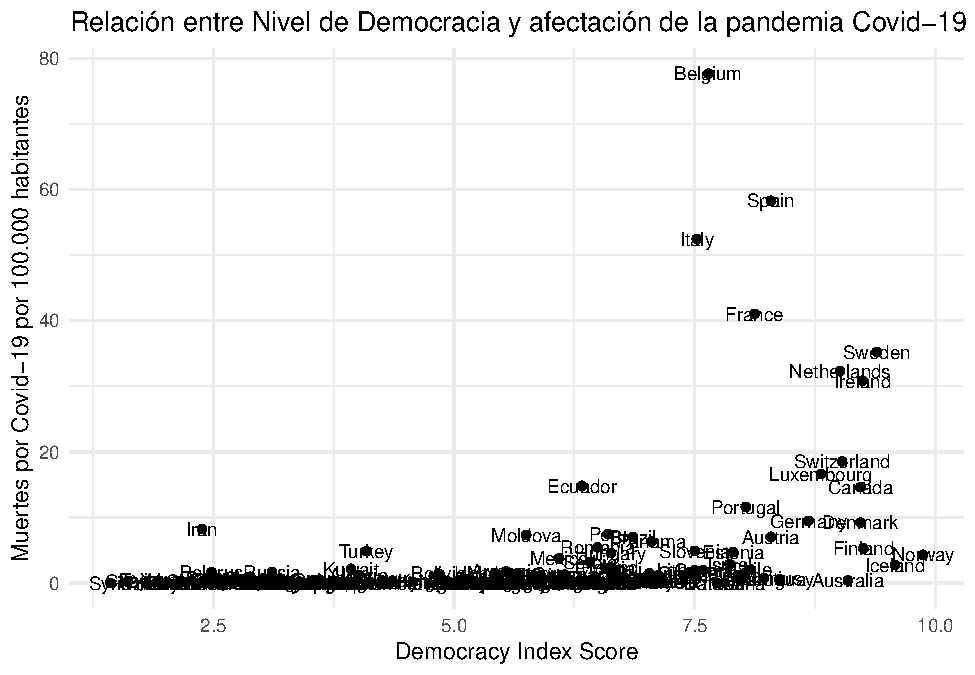
\includegraphics{2020-05-15-corrupcion-y-covid-19_files/figure-latex/unnamed-chunk-6-1.pdf}

En Europa:

\begin{Shaded}
\begin{Highlighting}[]
\NormalTok{lastrestablaseuropa <-}\StringTok{ }\NormalTok{lastrestablas }\OperatorTok\StringTok{ }\KeywordTok{filter}\NormalTok{(Continent}\OperatorTok{==}\StringTok{"Europe"}\NormalTok{)}

\NormalTok{p <-}\StringTok{ }\KeywordTok{ggplot}\NormalTok{(lastrestablaseuropa, }\KeywordTok{aes}\NormalTok{(Score, muertespor100000habitantes))}
\NormalTok{p }\OperatorTok{+}\StringTok{ }\KeywordTok{geom_point}\NormalTok{() }\OperatorTok{+}\StringTok{ }\KeywordTok{geom_text}\NormalTok{(}\KeywordTok{aes}\NormalTok{(}\DataTypeTok{label=}\NormalTok{Country), }\DataTypeTok{size=}\DecValTok{3}\NormalTok{) }\OperatorTok{+}
\KeywordTok{labs}\NormalTok{(}\DataTypeTok{title =} \StringTok{"Relación entre Nivel de Democracia y afectación de la pandemia Covid-19"}\NormalTok{) }\OperatorTok{+}
\KeywordTok{ylab}\NormalTok{(}\StringTok{"Muertes por Covid-19 por 100.000 habitantes"}\NormalTok{) }\OperatorTok{+}
\KeywordTok{xlab}\NormalTok{(}\StringTok{"Democracy Index Score"}\NormalTok{) }\OperatorTok{+}\StringTok{ }\KeywordTok{theme_minimal}\NormalTok{()}
\end{Highlighting}
\end{Shaded}

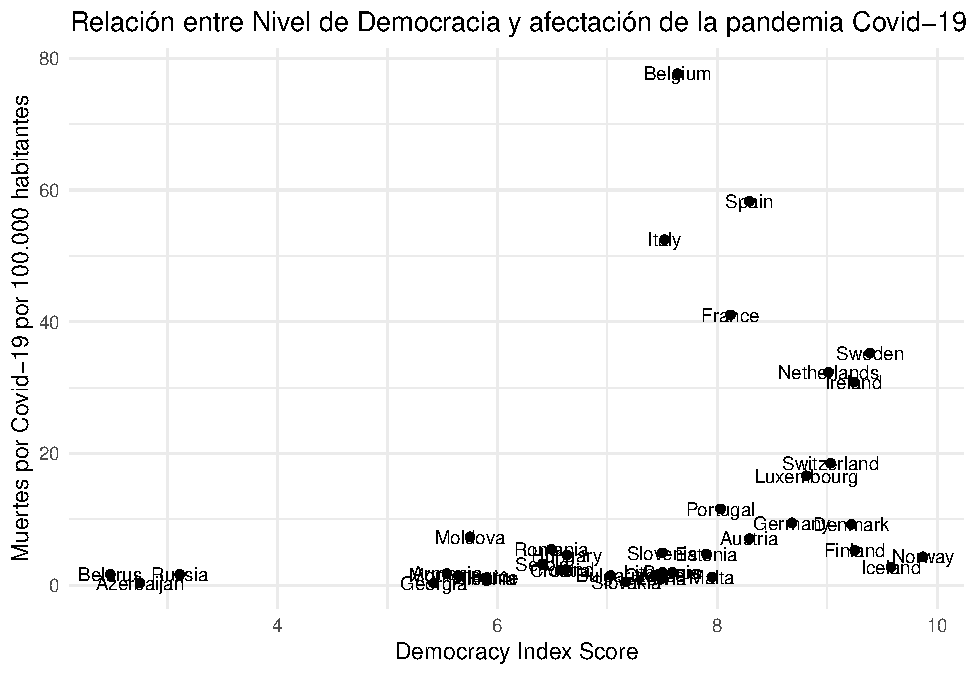
\includegraphics{2020-05-15-corrupcion-y-covid-19_files/figure-latex/unnamed-chunk-7-1.pdf}

Probemos de visualizar un correlograma de los indicadores que tenemos:

\begin{Shaded}
\begin{Highlighting}[]
\KeywordTok{library}\NormalTok{(ggcorrplot)}
\NormalTok{lastrestablas <-}\StringTok{ }\NormalTok{lastrestablas }\OperatorTok\StringTok{ }\KeywordTok{select}\NormalTok{(}\KeywordTok{c}\NormalTok{(}\StringTok{"Procesos electorales y pluralismo"}\NormalTok{, }\StringTok{"Gobierno funcional"}\NormalTok{, }\StringTok{"Participacion"}\NormalTok{, }\StringTok{"Cultura política"}\NormalTok{, }\StringTok{"Libertades civiles"}\NormalTok{, }\StringTok{"muertespor100000habitantes"}\NormalTok{))}
\NormalTok{corr =}\StringTok{ }\KeywordTok{cor}\NormalTok{(lastrestablas)}

\KeywordTok{ggcorrplot}\NormalTok{(corr, }\DataTypeTok{hc.order =}\NormalTok{ T,}
           \DataTypeTok{type =} \StringTok{"lower"}\NormalTok{,}
           \DataTypeTok{lab =}\NormalTok{T,}
           \DataTypeTok{lab_size =}\DecValTok{3}\NormalTok{,}
           \DataTypeTok{method=}\StringTok{"circle"}\NormalTok{,}
           \DataTypeTok{colors =} \KeywordTok{c}\NormalTok{(}\StringTok{"tomato3"}\NormalTok{,}\StringTok{"thistle"}\NormalTok{,}\StringTok{"springgreen3"}\NormalTok{),}
           \DataTypeTok{title=}\StringTok{"correlaciones"}\NormalTok{,}
           \DataTypeTok{ggtheme=}\NormalTok{theme_minimal)}
\end{Highlighting}
\end{Shaded}

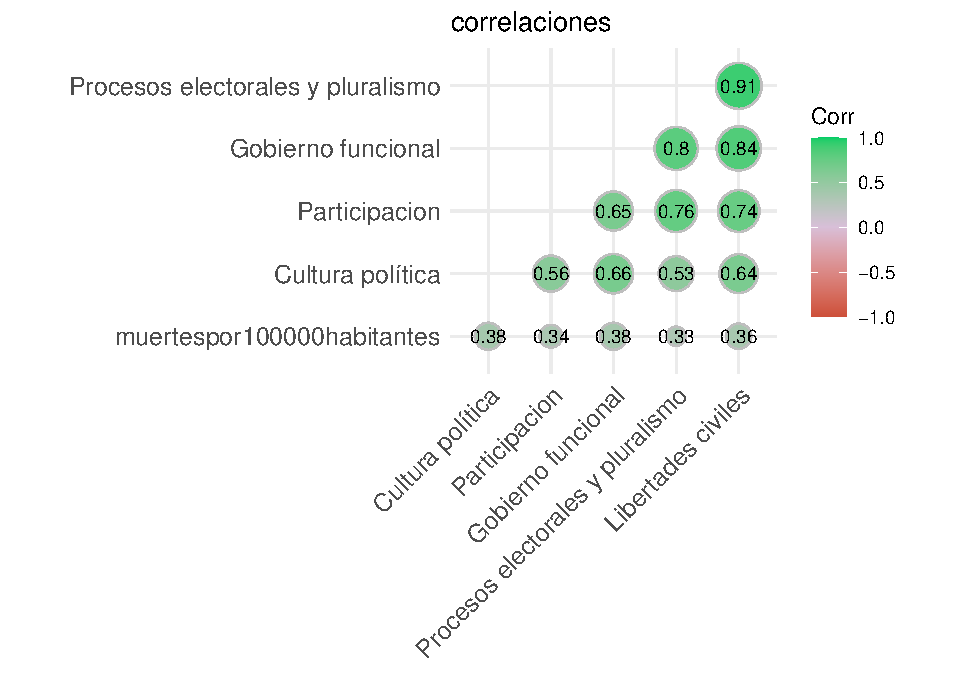
\includegraphics{2020-05-15-corrupcion-y-covid-19_files/figure-latex/unnamed-chunk-8-1.pdf}

Quizás el nivel de cultura política o el que el gobierno funcione pueda
afectar algo a como se gestiona una pandemia y en el número de muertes
producidas?

Veamos por países la correlación entre nivel Cultura política y muertes
por 100.000 habitantes:

\begin{Shaded}
\begin{Highlighting}[]
\KeywordTok{library}\NormalTok{(widyr)}
\NormalTok{cors <-}\StringTok{ }\NormalTok{lastrestablaseuropa }\OperatorTok\StringTok{ }\KeywordTok{pairwise_cor}\NormalTok{(Country, }\StringTok{"Cultura política"}\NormalTok{, muertespor100000habitantes)}
\NormalTok{cors }\OperatorTok\StringTok{ }\KeywordTok{arrange}\NormalTok{(correlation)}
\end{Highlighting}
\end{Shaded}

\begin{verbatim}
FALSE # A tibble: 1,482 x 3
FALSE    item1    item2    correlation
FALSE    <chr>    <chr>          <dbl>
FALSE  1 Slovakia Norway       -0.0833
FALSE  2 Norway   Slovakia     -0.0833
FALSE  3 Denmark  Norway       -0.0833
FALSE  4 Spain    Norway       -0.0833
FALSE  5 France   Norway       -0.0833
FALSE  6 Cyprus   Norway       -0.0833
FALSE  7 Hungary  Norway       -0.0833
FALSE  8 Poland   Norway       -0.0833
FALSE  9 Serbia   Norway       -0.0833
FALSE 10 Georgia  Iceland      -0.0833
FALSE # ... with 1,472 more rows
\end{verbatim}

\begin{Shaded}
\begin{Highlighting}[]
\KeywordTok{library}\NormalTok{(ggraph)}
\KeywordTok{library}\NormalTok{(igraph)}
\NormalTok{cors }\OperatorTok
\StringTok{  }\KeywordTok{filter}\NormalTok{ (correlation }\OperatorTok{>}\NormalTok{.}\DecValTok{4}\NormalTok{) }\OperatorTok\StringTok{ }
\StringTok{  }\KeywordTok{graph_from_data_frame}\NormalTok{() }\OperatorTok
\StringTok{  }\KeywordTok{ggraph}\NormalTok{(}\DataTypeTok{layout =}\StringTok{"fr"}\NormalTok{) }\OperatorTok{+}
\StringTok{  }\KeywordTok{geom_edge_link}\NormalTok{(}\KeywordTok{aes}\NormalTok{(}\DataTypeTok{alpha =}\NormalTok{ correlation, }\DataTypeTok{width =}\NormalTok{correlation), }\DataTypeTok{edge_colour =} \StringTok{"tomato3"}\NormalTok{) }\OperatorTok{+}
\StringTok{  }\KeywordTok{geom_node_point}\NormalTok{(}\DataTypeTok{size =} \DecValTok{2}\NormalTok{, }\DataTypeTok{color =}\StringTok{"black"}\NormalTok{) }\OperatorTok{+}
\StringTok{  }\KeywordTok{geom_node_text}\NormalTok{(}\KeywordTok{aes}\NormalTok{(}\DataTypeTok{label =}\NormalTok{ name), }\DataTypeTok{repel =}\NormalTok{ T) }\OperatorTok{+}
\StringTok{  }\KeywordTok{theme_void}\NormalTok{() }\OperatorTok{+}
\StringTok{  }\KeywordTok{labs}\NormalTok{(}\DataTypeTok{title =} \StringTok{"Correlación entre países, cultura política y número de muertes por covid-19"}\NormalTok{)}
\end{Highlighting}
\end{Shaded}

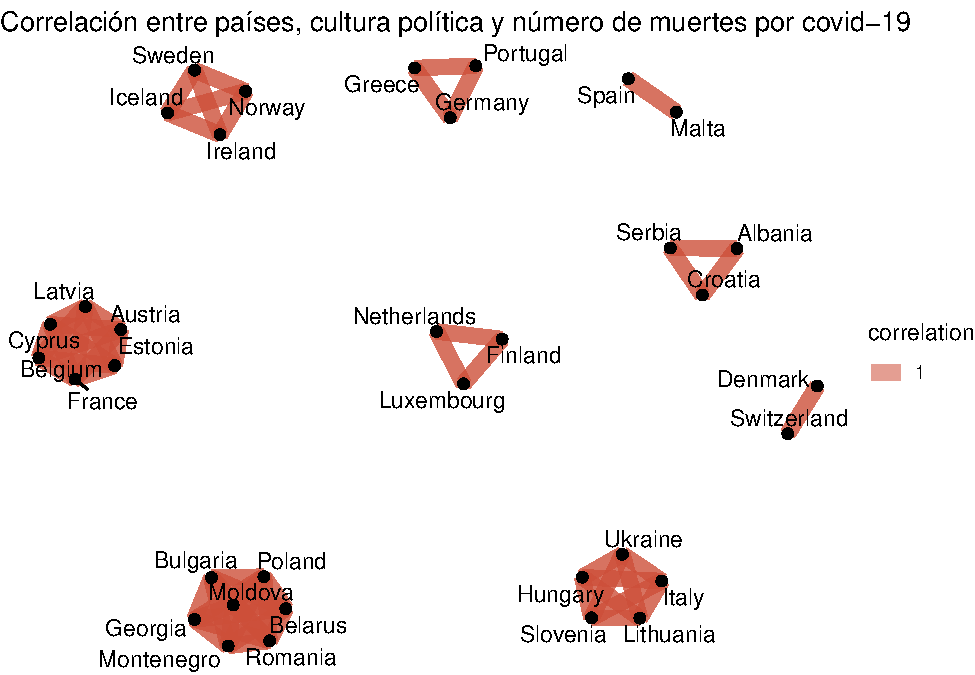
\includegraphics{2020-05-15-corrupcion-y-covid-19_files/figure-latex/unnamed-chunk-10-1.pdf}

Ahora observemos la correlación entre nivel Gobierno funcional y muertes
por 100.000 habitantes:

\begin{Shaded}
\begin{Highlighting}[]
\KeywordTok{library}\NormalTok{(widyr)}
\NormalTok{corsgf <-}\StringTok{ }\NormalTok{lastrestablaseuropa }\OperatorTok\StringTok{ }\KeywordTok{pairwise_cor}\NormalTok{(Country, }\StringTok{`}\DataTypeTok{Gobierno funcional}\StringTok{`}\NormalTok{, muertespor100000habitantes)}
\NormalTok{corsgf }\OperatorTok\StringTok{ }\KeywordTok{arrange}\NormalTok{(correlation)}
\end{Highlighting}
\end{Shaded}

\begin{verbatim}
FALSE # A tibble: 1,482 x 3
FALSE    item1      item2    correlation
FALSE    <chr>      <chr>          <dbl>
FALSE  1 Spain      Finland      -0.0556
FALSE  2 Portugal   Finland      -0.0556
FALSE  3 Estonia    Finland      -0.0556
FALSE  4 Finland    Spain        -0.0556
FALSE  5 Montenegro Spain        -0.0556
FALSE  6 Finland    Portugal     -0.0556
FALSE  7 Finland    Estonia      -0.0556
FALSE  8 Montenegro Latvia       -0.0556
FALSE  9 Georgia    Slovakia     -0.0556
FALSE 10 Montenegro Romania      -0.0556
FALSE # ... with 1,472 more rows
\end{verbatim}

\begin{Shaded}
\begin{Highlighting}[]
\KeywordTok{library}\NormalTok{(ggraph)}
\KeywordTok{library}\NormalTok{(igraph)}
\NormalTok{corsgf }\OperatorTok
\StringTok{  }\KeywordTok{filter}\NormalTok{ (correlation }\OperatorTok{>}\NormalTok{.}\DecValTok{4}\NormalTok{) }\OperatorTok\StringTok{ }
\StringTok{  }\KeywordTok{graph_from_data_frame}\NormalTok{() }\OperatorTok
\StringTok{  }\KeywordTok{ggraph}\NormalTok{(}\DataTypeTok{layout =}\StringTok{"fr"}\NormalTok{) }\OperatorTok{+}
\StringTok{  }\KeywordTok{geom_edge_link}\NormalTok{(}\KeywordTok{aes}\NormalTok{(}\DataTypeTok{alpha =}\NormalTok{ correlation, }\DataTypeTok{width =}\NormalTok{correlation), }\DataTypeTok{edge_colour =} \StringTok{"tomato3"}\NormalTok{) }\OperatorTok{+}
\StringTok{  }\KeywordTok{geom_node_point}\NormalTok{(}\DataTypeTok{size =} \DecValTok{2}\NormalTok{, }\DataTypeTok{color =}\StringTok{"black"}\NormalTok{) }\OperatorTok{+}
\StringTok{  }\KeywordTok{geom_node_text}\NormalTok{(}\KeywordTok{aes}\NormalTok{(}\DataTypeTok{label =}\NormalTok{ name), }\DataTypeTok{repel =}\NormalTok{ T) }\OperatorTok{+}
\StringTok{  }\KeywordTok{theme_void}\NormalTok{() }\OperatorTok{+}
\StringTok{  }\KeywordTok{labs}\NormalTok{(}\DataTypeTok{title =} \StringTok{"Correlación entre países, gobierno funcional y número de muertes por covid-19"}\NormalTok{)}
\end{Highlighting}
\end{Shaded}

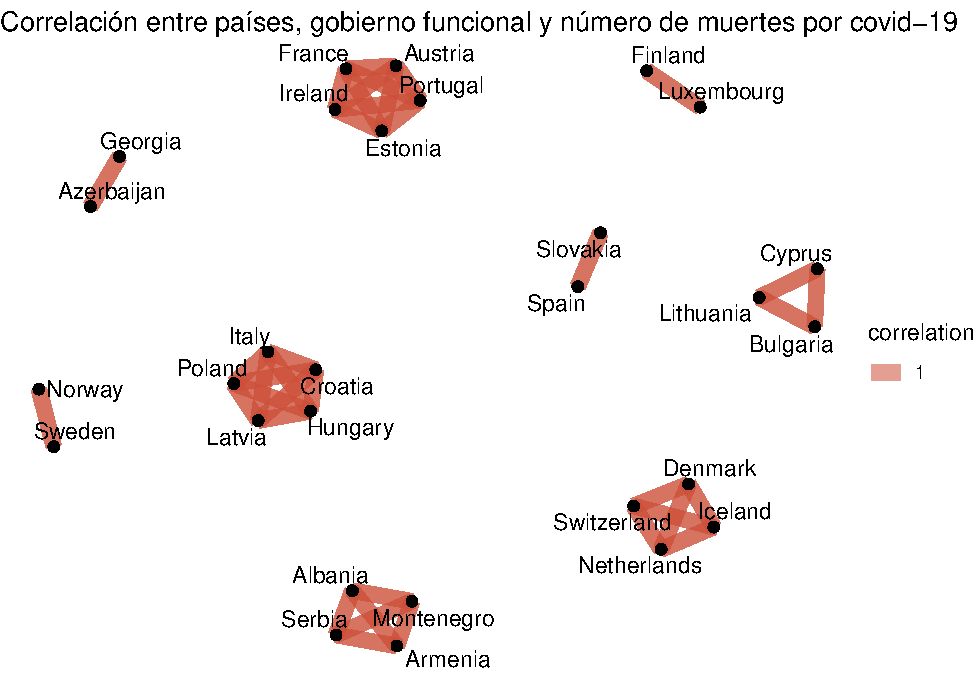
\includegraphics{2020-05-15-corrupcion-y-covid-19_files/figure-latex/unnamed-chunk-12-1.pdf}

\end{document}
